\section{Updates}

{\bf 2026-09-14 - } I think I have accumulated most of the various parts I will need for this simulation workflow. 

I have a notebook now that can make a simple map with input $C_\ell$ and place a point source at a specified RA/Dec. although the code says it is lon lat, but this is just a coordinate difference. So long as the simulated sky maker and the scanning use the same coordinates we should be fine.

\begin{figure}[h!]
    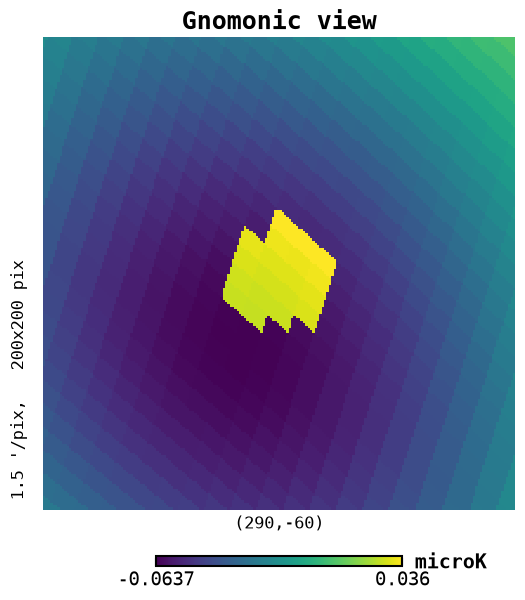
\includegraphics[width=0.6\textwidth]{Chapters/sim_point_source.png}
    \centering
\end{figure}

I can scan the simulated sky using TOAST:

\begin{figure}[h!]
    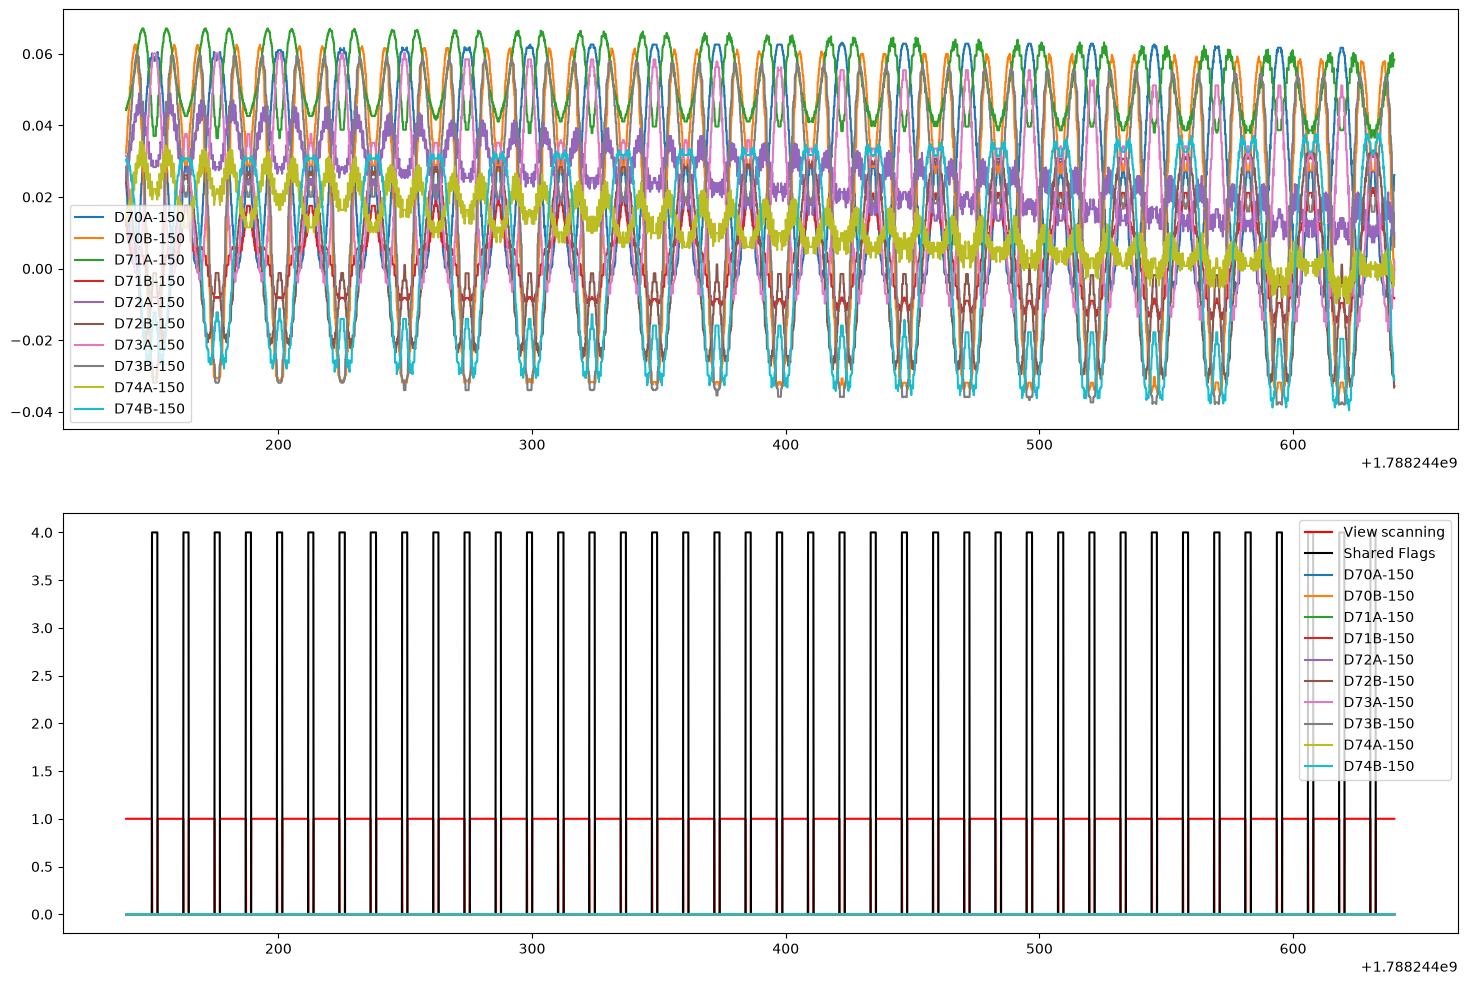
\includegraphics[width=0.8\textwidth]{Chapters/Scanned_PS.png}
    \centering
\end{figure}

And Claude helped decipher how to run the \verb+toast_so_map+ maximum likelihood mapmaker code to make a map from TOD. This process is now in a batch slurm job so I can easily re-run it.

\begin{figure}[h!]
    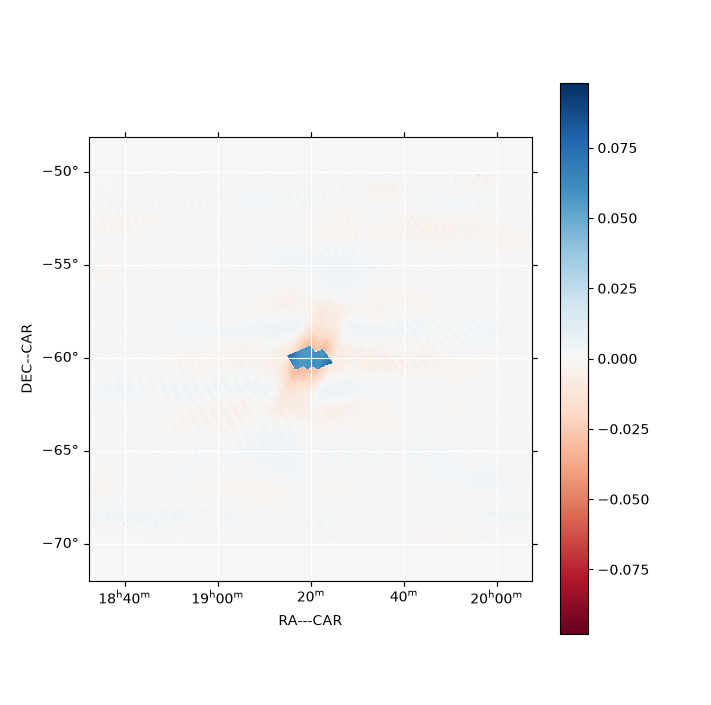
\includegraphics[width=0.7\textwidth]{Chapters/reconstructed_PS.png}\centering
\end{figure}

Oh and I can make a simple operator now!

\begin{figure}[h!]
    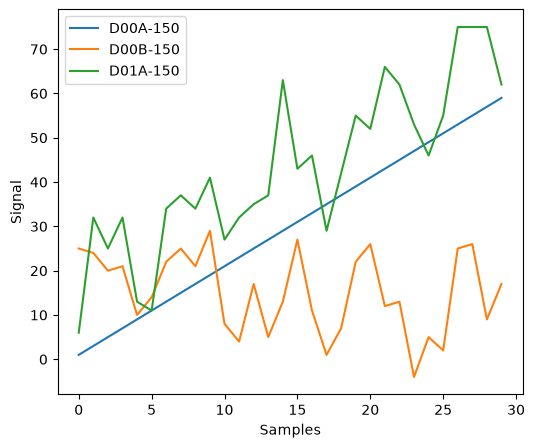
\includegraphics[width=0.7\textwidth]{Chapters/basicOperator.png}\centering
\end{figure}

Next Steps:
\begin{itemize}
    \item Look into the HWP wobble found in \verb+\sotodlib\sotodlib\toast\ops\hwp_wobble.py+
    \item Make a more realistic point source.
    \item Sim a more realistic LAT. 
\end{itemize}

{\bf 2026-09-18}
Made a rudamentary pointing jitter operator that is based on adding a sinusoidal pattern with random gaussian noise of the form:
 \begin{equation}
    \begin{split}
        \Delta \text{lon} = - A \sin{\nu t} - (\text{np.random.rand()}\delta_{az} - \delta_{az}/2) \\
        \Delta \text{lat} = A \sin{\nu t} + (\text{np.random.rand()}\delta_{el} - \delta_{el}/2) \\
        
    \end{split}
\end{equation}


\section{Run Notes}

To run with a pointing offset
\begin{verbatim}
    srun python run_toast_sim/toast_sim.py \
    sim_sky_maps/maps/map_with_3FWHM_source.fits \
    toast_tutorial/out_sim_ground/custom_map/test_schedule.txt \
    --load_telescope run_toast_sim/telescope.hdf5 \
    --pointing_offset \
    --out_dir "${OUT_DIR}" \
\end{verbatim}
then
\begin{verbatim}
    sbatch run_toast_sim/slurm_toast_sim.slurm <Name of OutDir>
\end{verbatim}

To run with a pointing jitter